\documentclass{article}
\usepackage{multirow}
\usepackage[utf8]{inputenc}
\usepackage{graphicx}
\usepackage{pdfpages}
\usepackage{url}
\usepackage{float}
\graphicspath{ {pictures/} }

\usepackage[utf8]{inputenc}
\usepackage[english]{babel}
 
\usepackage{amsthm}
 
\theoremstyle{definition}
\newtheorem{definition}{Definition}[section]
\begin{document}
\bibliographystyle{plain}

\begin{titlepage}
	\centering
	
\includegraphics{sussex} \par
	{\scshape\Large Final Year Project \par}
	{\Large\scshape BSc (Hons) Computer Science\par}
	{\Large\scshape 2017\par}
	{\scshape\Large Final Report\par}
	\vspace{1cm}
	{\huge\bfseries Distributed Graph Processing Using Apache Hadoop and Spark\par}
	\vspace{1cm}
	{\Large\itshape Kea Tossavainen \par}
	{\Large\itshape Candidate number: 132250\par}
	\vfill
	{\Large\itshape supervised by\par}
	{\Large\itshape George Parisis\par}

	\vfill
\end{titlepage}


\tableofcontents

\newpage
\section{Introduction}

\subsection{Big Data}
Current era of technology has changed the way we handle data. Unlike centuries before, technology has enabled the world to store data in virtual format rather than archiving decades worth of paper records. In current years, the amount of virtual data has been constantly growing and at the moment, according to IBM Big Data and Analytics Hub \cite{ibm}, "2.3 trillion gigabytes of data is created each day". The term for this important topic in Computer Science is Big Data; how to store, handle, process and calculate these amounts of data. Big Data includes user created data; videos and pictures uploaded to several social media sites and streaming sites, blogs and microblogs, but also data from companies like virtual backups and medical records. \\

IBM Big Data And Analytics Hub describes four dimensions of Big Data, four V's: volume, variety, velocity and veracity. Volume refers to the amount of data being created and stored. Variety is the dimensions of data created; data created by individual people but also by companies. Velocity refers to the analysis of streaming data and the speed of analysis. Veracity is the uncertainty and unreliability of data, for example Wikipedia as a source material when everyone can edit articles. \\

Big Data is an important topic, not only in the practical way how to store and process Big Data, but also how to harness it to research purposes. Big Data has enabled completely new fields and ways of research, for example sentiment analysis of new products and celebrities, social media research on social interaction and friendships like Degrees of Separation in Social Networks research by Bakhshandeh et al \cite{sixdegrees}, and research on networks. However, to use this amount of data, there is a real need for frameworks and systems that can handle the quantity of data without being extremely time consuming. For this project, several batch processing and distributed data processing frameworks and systems were explored and tested. \\

\subsection{Network processing}
Different type of networks, like social media networks, transport route networks and internet networks, are a big part of Big Data. Many practical and theoretical problems in Computer Science are related to networks. They are a highly researched topic and in research, networks are often mapped to graphs. These graphs are getting incredibly big; social media websites have millions of users and connections between them. Processing this data is time consuming and requires significant amount of computational power. Networks can be partitioned into smaller chunks, but sometimes the whole network has to be used. The goal for this project was to build a system using several Big Data tools to be able to do computations and run algorithms on graphs efficiently. This project is motivated by research from Tee, Parisis and Wakeman \cite{Tee2016b}. Their research about importance of a node in a graph uses node properties, concentrating on node entropy, to define most important nodes in a graph. In their research there is a need for a system that can run computations on large graphs. Their paper is further introduced in the background reading section of this report. \\

\subsection{This Report}
The rest of this report is as follows; professional considerations; acknowledgements, background reading and other sources; JUHUU HERE \\


\section{Professional Considerations}
This project adheres to BCS Code of Conduct. This project was within my professional competence being a project related to several topics studied during my degree of Computer Science. \\

This project didn't include any kind of personal or private data, and did not involve human participants. Datasets used in this project were taken from Stanford Snap \cite{snap}, which are real life graph datasets, but they have been anonymized before being published and thus do not contain personal information. \\

The programming interfaces and frameworks used in this project are Open Source and freely available for everyone. Any borrowed code will be referenced accordingly and all will be done considering copyrights and ownership of code. Papers, sources, websites and other information used are referenced. \\

\section{Acknowledgements}
A big thank you to the supervisor of this project, George Parisis, for his patience, help and supervision. This project is motivated by a research by Phil Tee, Ian Wakeman and George Parisis \cite{Tee2016b}. Thank you to Felix Bowman for teaching and helping with Scala programming language. Thank you to Hayden Tucker for all the support. \\ 

\section{Background reading and motivation}
A large part of this project consisted on getting to know several distributed and Big Data processing tools and systems. This was done reading and understanding several papers; Google's paper about Google File System (GFS) \cite{Ghemawat2003}, Google's cluster data processing tool MapReduce \cite{Dean}, Google's storage system Bigtable for managing structured data \cite{Chang}, Google's cluster management system Borg \cite{Verma}, Google's graph processing tool Pregel \cite{Malewicz2010}, Apache's cluster computation system Spark \cite{Zaharia2012} and paper by Tee, Parisis and Wakeman \cite{Tee2016b} about their research on node importance and vertex measures. Background knowledge on the systems used was crucial so they could be used to their full potential and to limit the number of errors in the code. 

\subsection{Apache Hadoop and related papers}
Apache Hadoop is a framework for distributed storage and processing of large datasets. Hadoop consists of a Hadoop Distributed File System (HDFS) which stores the data; MapReduce processing model which splits input data into smaller chunks and shares the chunks to be processed by nodes; Hadoop YARN resource manager which manages computing resources; and Hadoop Common which contains libraries and utilities needed by Apache Hadoop. HDFS and MapReduce are inspired by papers from Google about their Google File System (GFS) \cite{Ghemawat2003} and MapReduce \cite{Dean}. The building blocks of Apache Hadoop will be introduced top down in this report; first MapReduce, then Yarn, HBase and finally HDFS. \\ 

\begin{figure}[H]
\centering
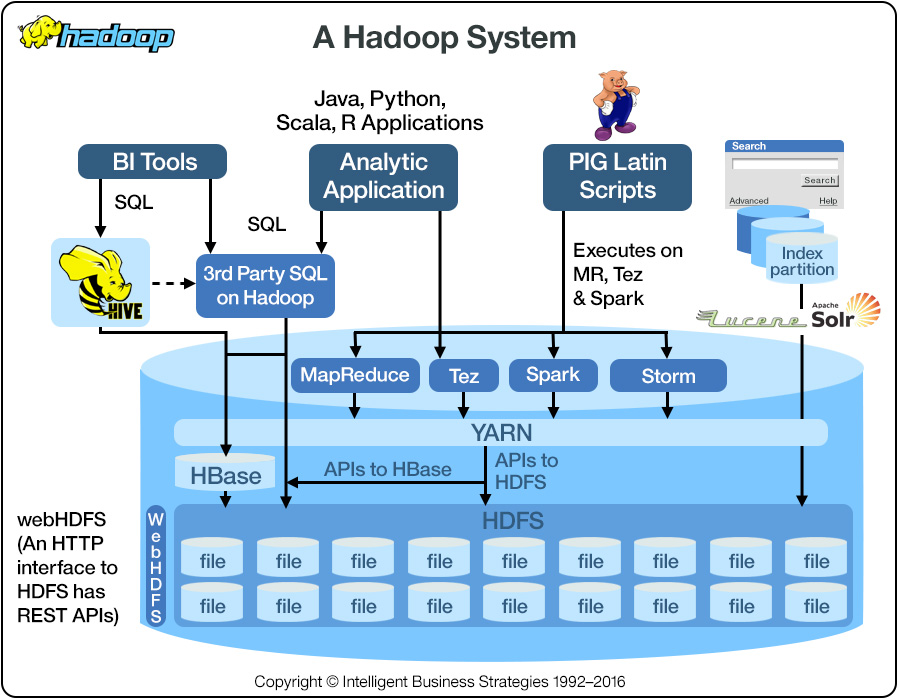
\includegraphics[scale=0.4]{SystemIllustration}
\caption{Hadoop System Illustration, from \cite{bmhadoop}}
\end{figure}

The paper \cite{Dean} by J. Dean and S. Ghemawat introduces Google's MapReduce. MapReduce processes data on large cluster and operates on sequences of actions. It takes an input formatted as a key, value -pairs, Map method maps these values to intermediate values, and Reduce method merges the intermediate values of a key to one value. Map and Reduce methods are user-defined and can be written to process different types of inputs. The idea behind MapReduce was to create a new abstraction that allows simple computations while hiding details like parallelisation, fault-tolerance and data distribution. \\

\begin{figure}[H]
\centering
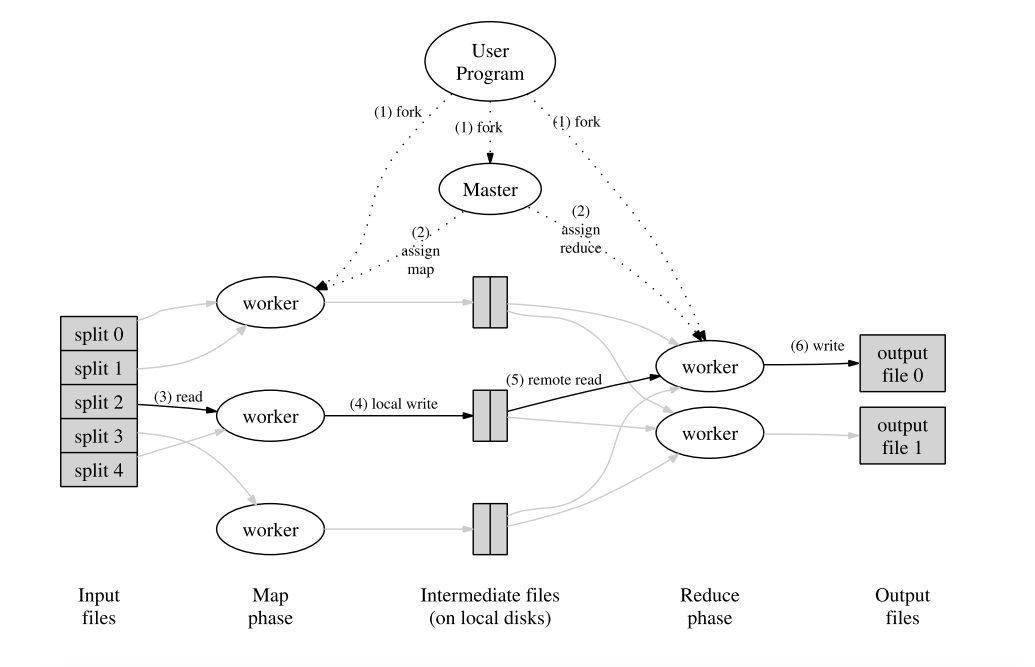
\includegraphics[scale=0.4]{mapreducefigure}
\caption{Map Reduce sequence of actions. }
\end{figure}

The MapReduce sequence of actions, shown in figure 2 (NOTE HERE CHECK IF RIGHT FIGURE NUMBER), starts by splitting the input file into M pieces and starts up copies on cluster machines. There are M Map tasks and R Reduce tasks. One of the copies is a master copy, which assigns Map and Reduce jobs to other clusters called worker clusters. Worker then reads its own input split, parses it into key, value -pairs and passes each to map method. The buffered pairs are then written into a local disk, which is partitioned into R regions. Locations of these pairs are passed back to the master cluster and master then assigns reduce operations to clusters by passing the location of the buffered data, which is sorted by keys. Workers iterate over keys and passes the values to Reduce operation. MapReduce sequence of actions returns exactly R outputs. 
MapReduce handles fault-tolerance by allowing master cluster to ping each of the worker cluster, and if the worker doesn't respond in a certain amount of time, the worker is marked as failed by the master and the task is assigned to another worker node. If a map task is completed or failed, they are marked as idle and become eligible for rescheduling. Because map task results are stored on local disks, even completed map tasks will be recomputed in a case of a failure. All workers working on reduce tasks will be notified of this re-execution and any worker working on a reduce task will read the data from the new worker. Master nodes write checkpoints to protect from master node failure. If a master node fails, a new copy will simply be started from the last checkpoint.
MapReduce can express many real world tasks, and examples they give in the paper is counting the number of occurrences of a word in a document, counting URL access frequency, distributed sort and others. They show that MapReduce can be used for several tasks while being computationally effective. MapReduce has further inspired other processing systems, like Apache GraphX Pregel's Send Message and Merge Message functions, which will be introduced later in this report. \\ 

Apache Hadoop's HBase is an open source version of Google's Bigtable, introduced in \cite{Chang}. Bigtable and HBase are storage systems for managing structured data. Both of these storage systems are designed for reliable scaling of petabytes of data and on thousands of machines. They resemble databases in several ways, but they provide a different interface. They have a simple model which supports dynamically controlling data layout and format, unlike databases which have full relational data models. The data model of Bigtable and HBase is described as "sparse, distributed, persistent, multidimensional sorted map", which is indexed by row and column keys and timestamp. This allows finding data on different attributes. Data is maintained in lexicographic order by row key and dynamically partitioned table is accessed by row range. Column keys are grouped into column families, and they form the basic unit access control. This allows access control, as well as memory and disk accounting, to be done on column-family level. Data organised by timestamps are organised in decreasing order, which allows faster access to newest data. 
Bigtable and HBase automatically handles garbage collection, and client-application can specify if only new-enough versions are stored by giving a timeframe or how many last versions are stored. 
Bigtable and HBase API's provides several functions for data handling. Table and column families support creation and deletion; clusters can be changed; table and column family metadata can be stored and access control rights can be edited. Client applications have rights to write and delete values, look up values and iterate over data. This means that data is accessible, and applications can decide how much data is stored. \\ 

In \cite{Verma} the authors introduce Google's Borg system, similar to Apache Hadoop's YARN. Borg, and YARN, are cluster managers, which allow running thousands of jobs at the same time. Borg combines admission control, efficient task-packing, over-commitment and machine sharing with process-level performance isolation to achieve high utilisation. Support for high-availability applications is given by runtime features that minimise fault-recovery time, and scheduling policies which reduce the probability of correlated failures. The main things Borg offers are a declarative job specification language, name service integration, real-time job monitoring and tools for analysing and simulating system behaviour. It hides the details of resource management and failure handling, which allows users to concentrate on developing their applications instead of unimportant details. Borg allows running workloads on tens of thousands of machines and consists of two types of services: long-running services that should not go down and batch jobs that take a few seconds to a few days to complete. 
Borg operates on jobs which have one or more tasks. Every job runs in a Borg cell, which is the core of Borg. Borg cell is a set of machines that work as a unit. The machines in a cell are connected by high-performance data center scale network fabric. The machine units or clusters usually have one large cell, but may also have smaller cells. The architecture of Borg cell consists of a set of machines, a Borgmaster, and an agent process Borglet. Borgmaster has two processes; scheduler and main Borgmaster. checkpointThe main Borgmaster process handles client systems that mutate state or provide read-only access to data. Main Borgmaster also manages state machines for all objects in the system, communicates with the Borglets and offers web UI. Borgmaster process is replicated five times to store in-memory copy of the state of the cell. This state is also recorded in highly-available, distributed store on the replicas' local disk. Borgmaster's state is stored in checkpoints in the form of a periodic snapshots, and a change log is stored in replicas' local disk. If a replica fails, during its recovery it dynamically re-synchronises its state from mother replicas.
All submitted job tasks are added to pending queue, which is scanned asynchronously by the scheduler. Scheduler then assigns tasks to machines if there are sufficient resources for the task. The scheduling algorithm has two parts; feasibility checking which finds the machines on which the task could run, and scoring which picks one of the machines which are feasible for the task.
Borglets are local Borg agents on every machine in a cell, and its job is to start and stop tasks, restart tasks if they fail, manages resources, rolls over debug logs and reports the state of the machine to Borgmaster. Borglets are polled by the Borgmaster every few seconds to retrieve the state of the machine and send any outstanding requests. If Borglet doesn't respond to several poll messages, the machine Borglet is on is marked as down and tasks will be rescheduled to other machines. If communication is restored, Borgmaster orders Borglet to kill the tasks to avoid duplicates.
All Borg tasks and jobs have properties that determine what resources they need, their priority, name, owner and other attributes. 
Borg uses priority and quota to choose jobs to schedule and run. Quota works in admission control, and decides the jobs that are admitted to scheduling, and priority decides which jobs to schedule. If there are more tasks than can be accommodated, higher priority tasks can obtain resources from lower priority tasks by killing the lowest priority tasks until the required resources are obtained. 
Googles's Frameworks and systems like BigTable and MapReduce run on top of Borg, just like on the open source version from Apache, HBase and MapReduce run on top of YARN. \\

GFS and its open source equivalent HDFS are scalable distributed file systems. Ghemawat et al introduce GFS in their paper \cite{Ghemawat2003}, and as the paper states, they have overcome a lot of issues that traditional file systems have when handling large amounts of data. GFS, and HDFS, were designed with several assumptions in mind: that the components of storage system are built of easily failing, inexpensive components; that there is no need to store and edit a number of large files; reading of the files is mostly either large streaming or small random reads; writing of the files is mostly large sequential appends to the file; that multiple clients concurrently append to the files; and that high bandwidth is required because client applications process data in bulk. Bulk processing means that there is no requirement for low latency in distributed file systems. Normal file systems have create, delete, read, write, open and close operations, but GFS also offers Snapshot and Record Append operations. Snapshot copies a file or a directory tree at low cost and Record Append allows concurrent appending from multiple clients.   
GFS architecture consists of a master server and multiple ChunkServers, which are accessed by client applications. The master stores the metadata information, but is not part of transmitting actual data. This allows the architecture to avoid bottlenecks forming and fast working in the one master server. The data is stored as fixed-size chunks in the ChunkServers, and the master holds the information about where the data is stored. The client application requests this information from the master, and then communicates directly with the ChunkServers. The master also handles garbage collection and periodically sends Heartbeats to each ChunkServer to confirm that they are still running.  \\

Even though Apache Hadoop and the underlying systems run hidden in the systems used for this project, this information was important for understanding how the systems are built, what they offer and how they work together. 

\subsection{Apache Spark}
Apache Spark \cite{Zaharia2012} is a cluster computing system, which runs on top of Apache Hadoop. Spark introduces a data structure, Resilient Distributed Dataset RDD, which allows parallel computation on distributed systems and implements good fault tolerance. One of the motivations for Spark was to provide abstractions for more general use than other systems have. Other systems, like Pregel and MapReduce for example don't allow users to load several datasets into memory, like Spark does. \\

Spark was built to efficiently handle iterative algorithms and interactive data mining tools. Most computing frameworks handle these applications really inefficiently, for example MapReduce allows large-scale data analytics, but is made inefficient because of the lack of abstractions for leveraging distributed memory. MapReduce and other frameworks create data, but don't allow easy reuse for the intermediate data, and this is important if the intermediate results are used by several parallel computations. To reuse the data, it has to be written to an external storage system, and this is waste of time and space due to data replication. Spark allows reusing the intermediate data, and optimises data placement while being fault tolerant. \\ 

Resilient Distributed Dataset RDD is a collection of elements, which can be of almost any type, and it is created by partitioning a dataset of these elements. Users can control the persistence and partitioning of RDD's. Users can choose which RDD's will be persisted in memory and choose the storage strategy for them. Partitioning and re-partitioning can be done based on a key or RDD's allow large scale, parallel computations on large clusters to be done in-memory. RDD's allow storing intermediate results while controlling data partitioning for optimised data placement. RDD's have comprehensive set of operators for manipulating stored data.  \\

Spark has two types of operations; transformations and actions like shown in figure 2. Transformations on RDD's return a new RDD and actions compute results. RDD's are not saved, but they can be persisted. This means that using transformations and actions on RDD's change the stored data, and the original or intermediate datasets might not be stored unless cache method is explicitly called on the RDD.\\

\begin{figure}[H]
\centering
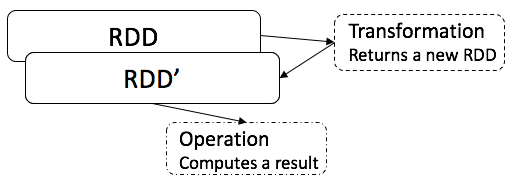
\includegraphics[scale=0.5]{RDD}
\caption{Sparks operations: transformations and actions}
\end{figure}

Spark has a number of operators, including Map, flatMap and Reduce. Map in Spark is a transformation and returns a new RDD, and Reduce is a action. Map is one-to-one mapping, while flatMap is similar to Map function in MapReduce. Some other relevant operators Spark has, and that are introduced in the paper, are partitionBy (transformation), which takes a partitioner and returns a new RDD which is partitioned differently, join and union (transformations), which take two RDD's and either unify them or join them. Some of these, like join are only available on RDD's of key-value pairs. \\

One important component in distributed processing is parallelisation. Because things run in parallel, variables and counters cannot be implemented without variables that are shared between all the clusters. Spark offers two types of shared variables; broadcast variables and accumulators. Broadcast variables are read-only variables, which are cached on each machine or cluster in serialised form, and can be used to share large quantities of data efficiently across partitions. Accumulators are variables that can be used to implement counters and sums.  \\ 

Even though core Spark can be used to implement graph processing algorithms, like page rank, Spark also has a graph processing component, which will be introduced later in this section of the report. 

\subsection{Pregel}
Pregel, introduced in \cite{Malewicz2010}, is a computational model suitable for efficient large scale graph processing, designed by Google for Google cluster architecture. The high-level organization of Pregel programs was inspired by Valiant's Bulk Synchronous Parallel model \cite{Valiant} and operates similarly to MapReduce. Pregel takes an input of a directed graph where each vertex has unique vertex identifier and associated with modifiable user-defined value and directed edges are associated with target vertices and consists of a modifiable user-defined value and target vertex identifier.

Pregel operates on sequences of iterations called supersterps. Within each superstep vertices compute in parallel, and each executed the same user-defined function, which is the logic of an algorithm and the function specifies the behaviour of a single vertex. Vertex can modify the state of its state or its outgoing edges' states, receive messages from previous superstep, send messages to other vertices for next superstep or even mutate the topology of the graph. The receivers of the messages a vertex sends does not have to be a neighbour of the sender vertex, however the identifier has to be known. A vertex can learn the identifier from earlier messages or the identifiers can be known for other reasons. If the destination vertex doesn't exist, a user-defined handler handles are executed. Depending on the algorithm and logic, the handler can, for example create a new vertex or remove an edge without a destination node. Pregel can terminate when vertices vote to halt, which means when the vertex is not in active state anymore. When vertex halts, it means that the vertex has no more work to do, unless triggered externally for example when receiving a message, and in which case vertex is reactivated. If a vertex is reactivated, it has to explicitly deactivate itself again. Algorithm terminates when there are no messages or all vertices are inactive simultaneously. 

The authors of the paper and the creators of Pregel chose a pure message passing model without remote reads because it is sufficiently expressive without remote reads and they have not found any graph algorithms for which message passing is insufficient. Message passing model also improves performance compared to models with remote reads. Since messages are delivered asynchronously in batches, latency is amortized. They chose to create this model instead of using series of MapReduce invocations for better usability and performance. They argue that since in chained MapReduce invocations would require passing entire state of the graph requires much more communication than message passing model where network is only used to transfer messages. 

Pregel has aggregators, which are a mechanism for global communication, monitoring and data. During a superstep, each vertex can provide a value to an aggregator, the system combines those values and the combined value will be available for all vertices in the next superstep. There are many uses for aggregators, for example statistics, global coordination or if there is a need to choose a vertex to play a distinguished role in an algorithm. Aggregators can be normal aggregators, which reduce input values from a single superstep or they can be sticky aggregators, which uses input values from all supersteps. 

Pregel partitions vertices based solely on the vertex ID and outgoing edges of that vertex. This implies that it's possible to know to which partition a given vertex belongs even if the vertex is owned by a different machine or if it doesn't exist yet. However, users can replace the default partitioning function. 

Pregel achieves fault tolerance similarly to Borg, through checkpoints. At the beginning of a superstep, the master tells workers to save the state of their partitions to persistent storage. This state includes vertex values, edge values and incoming messages. Aggregator values are stored by the master. Worker failures are detected using regular pinging from master to workers and if master doesn't hear back from the worker, the worker process are marked as failed. When one or more workers fail, the current state of the partitions assigned to these workers is lost and the master reassigns graph partitions to currently available workers, in which case they all reload the most recent checkpoint. 

\subsection{Apache GraphX}
For this project, both Giraph \cite{giraph} and GraphX \cite{GraphX} were considered. Even though, according to study by Facebook \cite{fbcase}, Giraph performs better and is more memory-efficient, GraphX was chosen because it's built on top of Spark, operates on RDD's and includes several already implemented algorithms, which have proven to be useful for this project. GraphX offers more in terms of computational possibilities while Giraph is more of an extended version of Pregel \cite{Malewicz2010}. However, if the aims of this project was to create a production-scale system, Giraph should be considered due to its efficiency. \\

GraphX is a component of Spark for graph processing and allows graph-parallel computation. As it's built on top of Spark, it extends the operations and operators in Spark and adds additional operators for Graph processing.  \\

GraphX represents a graph as Vertex and Edge RDD's. The created graph is directed property graph, which means that edges have directions and there are properties attached to each edge and vertex.  A vertex consists of a vertex id and a user-defined vertex property, and an edge consist of source and destination id's and a user-defined edge property. For this project, directed graph wasn't a necessity \\

GraphX has multiple algorithms already implemented, and these can be called for different graph processing tasks just like any other method or function is called. These algorithms include Pagerank, Label Propagation, Connected Components, Triangle Counting and previously mentioned Pregel, and they can be used further to implement other calculations. \\

\begin{figure}[H]
\centering
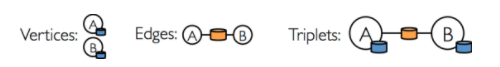
\includegraphics[scale=0.7]{/triplet}
\caption{Comparison of vertices, edges and triplets, from \cite{GraphX} }
\end{figure}

GraphX also offers triplet view for the graph. Triplet, shown in figure 3., consist of source vertex, source attribute, destination vertex, destination attribute and edge attribute. These are accessible through triplet. \\

There are several differences between Google's Pregel and GraphX's implementation of Pregel. Unlike Pregel, messages are computed in parallel as a function of the edge triplet and the message computation has access to both the source and destination vertex attributes. Vertices that do not receive a message are skipped within a super step. The Pregel operator terminates iteration and returns the final graph when there are no messages remaining. This is different than Google's Pregel computation model, which terminates when every vertex votes to halt. Also unlike in Pregel, GraphX's Pregel function doesn't allow changing the edge state since it operates on triplets, and it doesn't mutate the topology, only vertex properties. Another difference between GraphX's Pregel operator and Google's Pregel framework is the output. GraphX's Pregel always outputs a graph and Google's Pregel outputs set of values explicitly output by vertices, which can be an isomorphic graph to the original graph, but can also be modified or for example statistics on the graph. Because GraphX's Pregel's send message function works on triplets, the messages are always sent to neighbour vertices. This is not the case in Google's Pregel where the receiving vertex does not have to be a neighbour of the sender vertex. \\

Apache Spark's GraphX Pregel operator was used in the implementation of this project, and it will be outlined in section 6.1. of this report. \\

\subsection{Graph Entropy Measures}
The motivation for this project comes from research by Tee, Parisis and Wakeman \cite{Tee2016b}. Their research concentrates on identifying important and critical nodes in a network so, in case of a failure, the root cause can be identified. The goal for their research is to be able to determine vulnerable nodes in a network to be used in fault localisation. The research concentrates on vertex measures rather than measures on the whole graph. \\

They have considered a class of measures based on three different entropy measures: Structural, Chromatic and Von Neumann entropies. However, these measures require NP-Hard calculations over a whole graph, which doesn't scale for modern graphs which are large. Due to the scalability issues, their research is concentrating on Graph Entropy measures, concentrating on graph entropy for a single node. Their research shows, that calculating node entropies for the whole graph approximately gives the same results as entropy for a whole graph.  \\

WRITE MORE HERE

\begin{figure}[H]
\centering
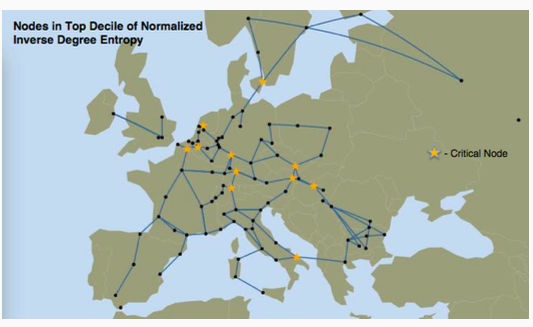
\includegraphics[scale=0.6]{nodeimportance}
\caption{Critical nodes in a network, figure 9 from \cite{Tee2016b}.}
\end{figure}

The figure above shows critical nodes identified by Normalized Degree Entropy. 

\subsection{Other sources of information}
\cite{hadooprealworld} has video tutorials and courses, which have proved useful while getting to know Hadoop. It offers courses and projects that can be done using Apache Hadoop. Hadoop in Real World website is created by engineers who have worked with Apache Hadoop in their professional careers. 
Another great resource for understanding Hadoop is IBM's Big Data \& Analytics Hub Blog's "What is Hadoop?" \cite{ibmhadoop} article. \\

Even though the Internet is full of information, GraphX is not widely enough used that there are not many sources or examples of more complex uses of GraphX. Main source of information was GraphX Programming Guide \cite{GraphX}. Book from Rinda Ramamonjison \cite{graphxbook} has been extremely valuable in getting to know GraphX and how to use it. Cake Solutions have done an example of usage GraphX Pregel functions in \cite{cakesolutions}, which proved to be useful while getting further knowledge of Pregel and how it can be used. \\

The test data was downloaded from Stanford Snap \cite{snap}, which contains anonymised network datasets. The Stanford Snap is a network analysis and graph mining library, and they have over 50 large network datasets, which include social networks, web graphs, road networks and other types of networks. \\

\section{Graph Processing}
This section consist of detailed information about the project. First this section outlines the goals of the project, then concentrates on the implementation, starting with an overview, used systems and then detailed explanation about the implementation. 

\subsection{Aims of the project}
The main goal for this process was to design and implement algorithms to process large amounts of data. In the early state of the project, objectives were identified as: 
\begin{itemize}
\item To learn about batch processing tools and graph processing tools
\item To gain knowledge and understanding about graph properties
\item To implement and design algorithms to process graph properties
\item To create a system to process different graph inputs
\item To improve processing time of calculations on graphs
\end{itemize}

When deciding requirements for this project, a program or system built in Java programming language was identified as a requirement. However, due to GraphX not having proper Java support, Scala was chosen as the main programming language for this project. This gave new challenges for the project due to lack of previous Scala knowledge. \\

Due to time constraints, proper evaluation for processing time wasn't done, so improving time of calculations was not something that was tested.  

\subsection{Overview of the implementation}
Substantial part of the implementation of this project was to use GraphX's Pregel function to create a j-sphere. J-sphere is a vertex's neighbourhood including all the vertices j hops away. Creating 1-sphere is simple and fast, it includes the vertices that source vertex is connected straight with an edge. In \cite{Tee2016b}, Tee, Parisis and Wakeman define j-sphere:

For a node $v_{i} \in V$, `j-sphere'
  centered on $v_{i}$ as:
\begin{equation}\label{eqn:jsphere}
S^{j}_{i}= \{ v_{k} \in V | d(v_{i},v_{k}) \leq j, j \geq 1 \} \cup \{ v_{i} \}
\end{equation}

They also define the related 'j-edges' $E^{j}$ as
\begin{equation}
  E^{j}_{i}=\{ e_{kl} \in E | v_{k} \in S^{j}_{i} \mbox{ and  } v_{l} \in S^{j}_{i} \}
\end{equation}

After implementing j-sphere with Pregel, goal was to implement several different algorithms to run on the j-sphere. 

Clustering coefficient, which was implemented using simple arithmetic expressions in Scala, is defined as: 
\begin{equation}
C_{i} = \frac{|2E_{i}|}{d(d+1)}
\end{equation}
Clustering coefficient captures how well meshed in its neighbourhood a vertex is. Clustering coefficient is crucial function in Tee, Parisis and Wakeman research. It is used to calculate Normalized Inverse Degree Entropy, which is defined as:
\begin{equation}
NVE(v_{i}) = \frac{1}{C_{i}} \times VE(v_{i})
\end{equation} 

The issues with implementation are discussed later in this section. 

\subsection{Used systems}
The systems and tools used for this project were:
\begin{itemize}
\item Apache Spark
\item Apache Spark GraphX
\item Scala Programming language
\item IntelliJ IDEA CE development environment
\item Datasets for testing were downloaded from Standford Snap
\end{itemize}

\subsection{Creating a JSphere}

For this project, two algorithms to create j-sphere, defined in equation 1, was implemented: naiveJSphere method, which takes a source vertex and creates a j-sphere only for that vertex, and jSphere method which creates a j-sphere for all the vertices in the graph. These algorithms were designed with the project supervisor George Parisis. Both methods use GraphX's Pregel API \cite{GraphX}. \\

Pregel operates on supersteps based on three user-defined functions: vertex program, send message and merge message. Vertex program determines what happens to received messages, send message determines which node messages are sent to and merge message merges two messages. Send message and merge message are analogous to MapReduce's Map and Reduce functions. Another parameters Pregel takes are initial message, which will be processed by first iteration of vertex program, maximum iterations and edge direction. Initial message is discarded after it's processed, and send message method creates new messages during each iteration. Maximum iterations, as self explanatory as it is, is set to be j. Because for this project edge direction doesn't matter, the edge direction was set to both. \\

The method naiveJSphere sends the initial message to all vertices in the graph with starting vertex ID, and vertex property for the start vertex is changed to true, in figure 5. Pregel then sends messages to the neighbouring vertices of the start vertex, and changes their attributes to true. This is done j + 1 times. GraphX offers a subgraph method, which takes edge predicate and vertex predicate, and creates a subgraph of vertices whose attribute is true and edges whose source and destination vertices are set true. 

\begin{figure}[H]
\centering
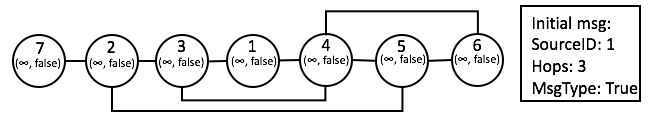
\includegraphics[scale=0.6]{/pregel/1}
\caption{Naive j-sphere: Initial Graph}
\end{figure}

\begin{figure}[H]
\centering
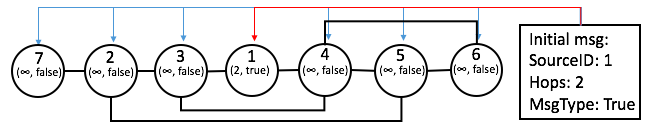
\includegraphics[scale=0.6]{/pregel/2}
\caption{Naive j-sphere: Initial Message sent to all nodes}
\end{figure}

\begin{figure}[H]
\centering
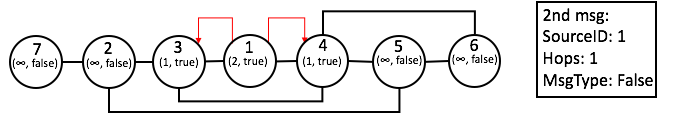
\includegraphics[scale=0.6]{/pregel/3}
\caption{Naive j-sphere: Message sent to 1 hop away from initial nodes}
\end{figure}

\begin{figure}[H]
\centering
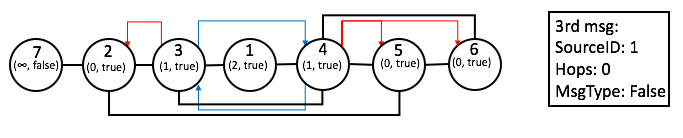
\includegraphics[scale=0.6]{/pregel/4}
\caption{Naive j-sphere: Messages ignored by nodes already visited}
\end{figure}

\begin{figure}[H]
\centering
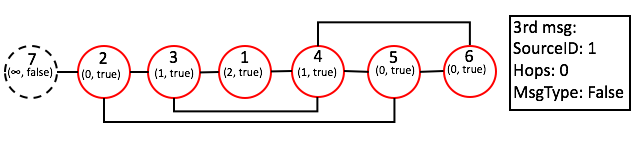
\includegraphics[scale=0.6]{/pregel/5}
\caption{Naive j-sphere: Subgraph created of nodes 2 hop away}
\end{figure}

The second j-sphere method creates a j-sphere for all vertices and 

\subsection{Implemented algorithms}

\textbf{Clustering coefficient} \\
Clustering coefficient, defined in equation 3, was simple to implement, since GraphX's Graph class has .numEdges function, which gives the number of edges in a given graph in Long datatype. This method takes a graph as a parameter, which allows it to be used in any graph created by the program, not just the result graph of the j-sphere method. \\

\textbf{}

\textbf{}

\textbf{}



\subsection{Issues in implementation and solutions for them}
The implementation of j-sphere had several issues. Because the graph was created from a file, the vertex attribute was set as an int, but j-sphere implementation required vertex attribute to store a state wether or not the vertex had been visited and how many hops away from the source node the vertex is. The solution to this was to create a second VertexRDD from the edges and associate a tuple for each vertex. This tuple was initialised as (0, false) for each node. This allowed easy use for the subgraph method, but it is not the most computationally effective way to create a graph. 
Another issue with j-sphere was to keep count of the hops. Because the user-defined functions in Pregel are called in parallel for each (active) vertex, having a simple variable to keep track of the hops was virtually impossible. One solution for this would've been to use GraphX's method for collecting neighbour vertices or vertex ids, which returns a Scala Sequence collection of Arrays or ID's or vertices. However, trying this approach, the program got stuck and even though it ran and no errors came up, the lookup method to lookup vertices in the collection seemed to not work. This approach was thus abandoned. The hop count was implemented with passing the hops through messages instead of storing it in a variable. 
GraphX operating on directed graphs also created its own issues. Even though GraphX's Pregel method takes EdgeDirection parameter, this only controls which direction the messages are received, not which direction the messages are sent. There were three ways to work around directed graphs, either create another EdgeRDD with all the edges reversed and add that to the graph on which Pregel will be called on, call the Pregel method twice, once for the original graph and then to a graph with same edges reversed, or having an if-statement to send messages to both sides depending on which direction the message comes from. First and second solutions are obviously computationally ineffective, especially for large graphs. The third solution was used to implement j-sphere.




\section{Conclusion}
-Is it fast? Does it work? What's happening
-What future work could include
-Was there any point in this? 

To utilise the systems used for this project requires detailed background research and for a one-off use it takes time and effort to implement something using these systems. However, these concepts and systems are widely used by companies, and knowledge of them is worthwhile. 

Looking back, more research should have been done when choosing the systems, and if there is future for this type of project, Apache Giraph might be more suitable for this type of distributed processing. 

\addcontentsline{toc}{section}{References}
\bibliography{fyp-final-report.bib.bib}

\section{Appendix}

\subsection{Meeting logs}

\subsection{Code snippets}
-Reference these in Programming and stuff if needed 

\end{document}